\chapter{Data Parallelism}
\begin{itemize}
    \item The phenomenon in which the \textbf{computation work of different parts of a dataset can be performed independently} of each other and thus can be executed in \textbf{parallel}.
    \item A large problem can be decomposed into \textit{n - smaller problems which can be executed independently. } This entails (re-)organizing the computation around the data such that the resulting computation can be executed in parallel to complete the overall job faster.
    \item Examples:
          \begin{itemize}
              \item Conversion of image from \textcolor{red}{R}\textcolor{green}{G}\textcolor{blue}{B}  $\rightarrow $ \textcolor{gray}{Gray} as visualized in \ref{fig:dp-rgb-gray-flowchart}.  Here each $\mathit{O}[0]\text{,} \mathit{O}[1]\text{,} \dots \mathit{O}[N-1]$ can be calculated independently.
                    \begin{figure}[!h]
                        \centering
                        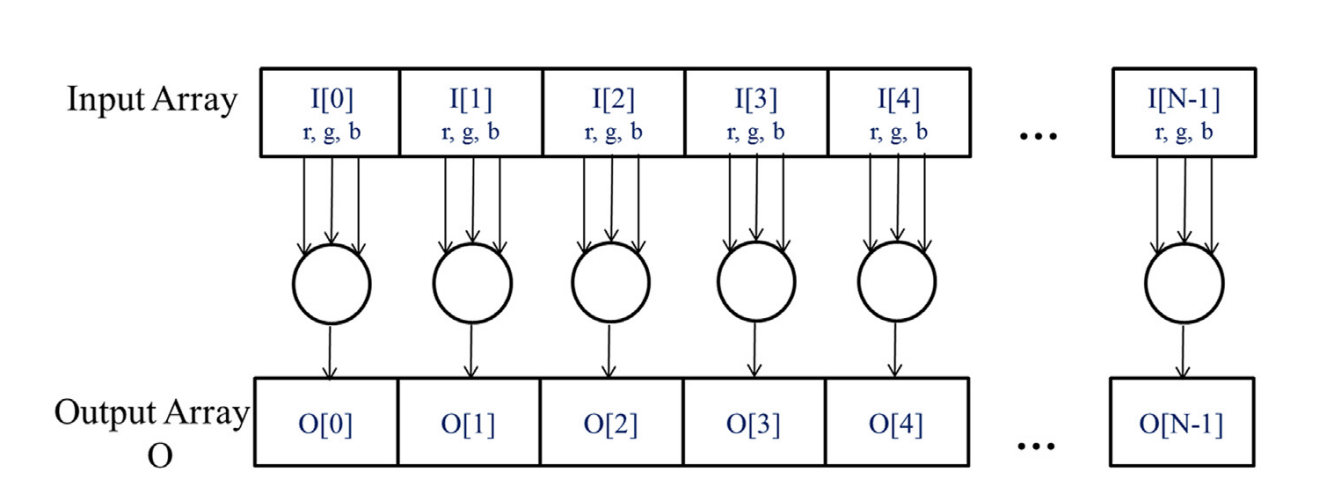
\includegraphics[width=0.7\linewidth]{Images/DP/rgb_to_gray_dataParallel.png}
                        \caption{Data parallelism of RGB-to-grayscale. Each pixel can be independently converted to grayscale}
                        \label{fig:dp-rgb-gray-flowchart}
                    \end{figure}
          \end{itemize}

\end{itemize}

\section{CUDA program structure}
\begin{itemize}
    \item CUDA C $\rightarrow$ Extends ANSI C language with minimal new syntax and library functions.
    \item Enables programmers to target heterogeneous computing systems containing both CPU and GPUs.
    \item \textit{host: } CPU ,  \textit{device}: GPU
    \item Each CUDA C file can be a mixture of \textit{host} code and \textit{device} code.
    \item Simplified CUDA program execution:
          \begin{itemize}
              \item Execution of host code (CPU serial code).
              \item Call of Kernel function $\rightarrow$ A large number of threads are launched on \textit{device} to execute kernel. (Collection of threads: \textit{grid}. )
              \item When all the threads of the grid finish execution, grid terminates $\rightarrow$ Execution on host continues until the next kernel is called.
                    \begin{figure}[!t]
                        \centering
                        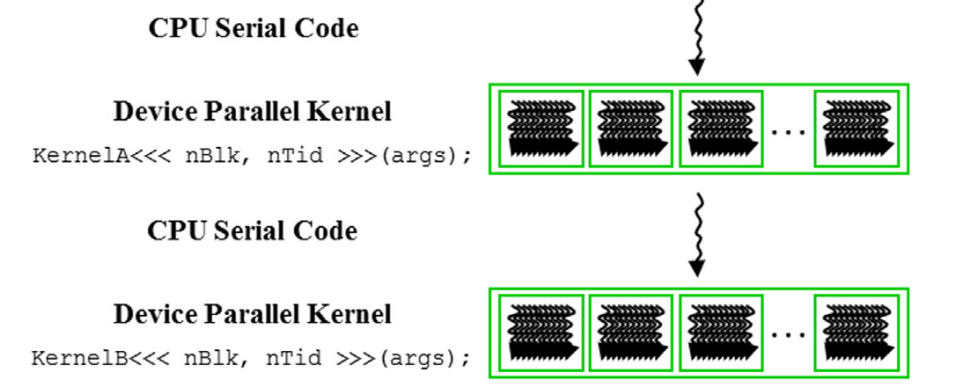
\includegraphics[width=0.75\linewidth]{Images/DP/cuda_exec.png}
                        \caption{Simplified execution of a CUDA program with no CPU and GPU overlap}
                        \label{fig:dp_cuda_exec}
                    \end{figure}
          \end{itemize}
    \item In the case of RGB $\rightarrow$ Gray conversion, each thread can be used to convert one pixel of the image to grayscale. In such case, the number of threads launched $\equiv$ number of pixels in the image.
    \item The threads in GPU take very few clock cycles to generate and schedule, as compared to traditional CPU threads, which typically take thousands of clock cycles to generate and schedule.

    \item The suffix \enquote{\texttt{\_h}} indicates the variables on host(CPU) and \enquote{\texttt{\_d}} to indicate the variable resides on device(GPU).
    \item The error-prone regions should be surrounded with the code that catches the error condition to print it out. For example, to catch the errors occuring during the memory allocation on device using \texttt{cudaMalloc()} function:
\end{itemize}
\begin{code}
    \captionof{listing}{Error catching for Malloc}
    \begin{minted}{cpp}
        // Error handling while allocating 'size' bytes of memory for pointer 'A_d'. Catch the return value of cudaMalloc() in err.
        cudaError_t err = cudaMalloc((void **)&A_d, size);
        // If enum 'err' is not equal to cudaSuccess, then print the error type, error name, in which file and line number.
        if (err != cudaSuccess){
            printf("%s: %s in %s at line %d\n",cudaGetErrorName(err), cudaGetErrorString(err), __FILE__, __LINE__);
            exit(EXIT_FAILURE);
        }
\end{minted}

\end{code}
\section{Kernel functions and threading}
\begin{itemize}
    \item Kernel function specifies the code to be executed by all threads during the parallel phase. $\rightarrow$ Since all the threads execute the same code, CUDA C programming is an instance of \textit{single-program multiple-data} \textbf{SPMD} parallel-programming style.
    \item Kernel call $\rightarrow$ launch of grid of threads. The threads are organized into two-level hierarchy.
          \begin{itemize}
              \item Grid: Organized into array of \textit{thread blocks} or \textbf{Blocks}.
              \item Block: All blocks of the grid are of same size; each block \textbf{can contain \textit{up to} 1024 threads}.
              \item Total number of threads in each block is specified in the host code.
          \end{itemize}
    \item The built-in variables that enable thread to distinguish itself from other are:
          \begin{itemize}
              \item \texttt{blockDim}: \textit{Build-in variable} specifying the number of threads in a block. Struct with 3 unsigned integer fields (\textit{x}, \textit{y} and \textit{z}), enabling one to organize threads into one-(x), two-(x, y) or three-dimensional(x, y, z) array.
              \item \texttt{blockIdx}:  Struct with 3 unsigned integer fields (\textit{x}, \textit{y} and \textit{z}). Gives all threads in a block a common block coordinate.
              \item \texttt{threadIdx}: Struct with 3 unsigned integer fields (\textit{x}, \textit{y} and \textit{z}). Gives each thread a unique coordinate within the block.
          \end{itemize}
    \item \textbf{Unique identifier for a thread} is calculated as:\\\texttt{data\_index=blockIdx.x * blockDim.x + threadIdx.x}
          \begin{figure}[H]
              \centering
              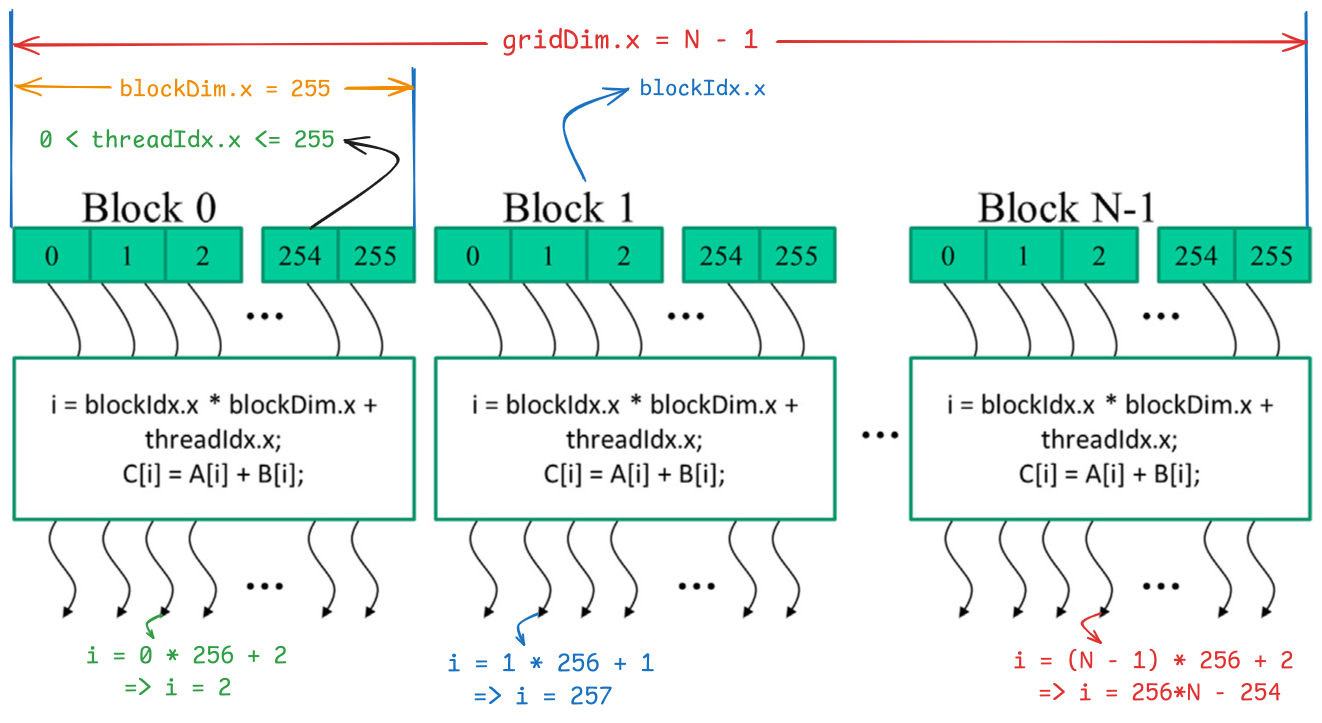
\includegraphics[width=.85\linewidth]{Images/DP/hierarchy_of_kernel.png}
              \caption{Hierarchy and organization of threads in a Grid}
              \label{fig:dp_hierarchy}
          \end{figure}

\end{itemize}

\section{\texttt{\_\_host\_\_,\_\_global\_\_ and \_\_device\_\_ } keywords}
\begin{itemize}
    \item \texttt{\_\_host\_\_}: Indicates that the function being declared is a CUDA host function. Is a function that is \textbf{executed on the CPU}. By default, all functions in CUDA are \textsl{host} functions, if not specified otherwise.
    \item \texttt{\_\_global\_\_}: Indicates the function being declared is a \textbf{CUDA C function}. Such a kernel function is \textbf{executed on the device and can be called from the host}. This keyword indicates that the function is a kernel and that it \textbf{can be called to generate a grid of threads on a device}.
    \item \texttt{\_\_device\_\_}: Indicates that the function being declared is a \textsl{CUDA device} function. This function \textbf{executes only on device, can be called only from a kernel function or another device function}. The device function is executed by the device thread that calls it and does not result in any new  device threads being launched.
    \item \textbf{\textit{NOTE}}: One can use both  \texttt{\_\_host\_\_} and \texttt{\_\_device\_\_} keywords in a function declaration. $\implies$ Two versions of the object code is compiled for same function. $\rightarrow$ One is a pure host function (call, execution) and the other is pure device function. Supports the common use case when the same function source code can be recompiled to generate device version. Ex. user-library functions.
\end{itemize}

\begin{center}
    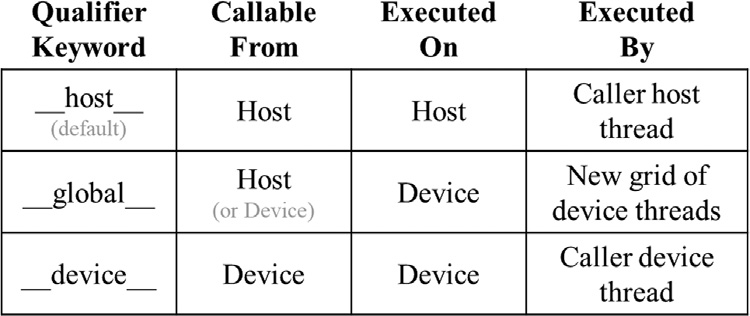
\includegraphics[width=0.7\linewidth]{Images/DP/cuda_keywords.png}
\end{center}

\begin{code}
    \captionof{listing}{Declaration of a simple kernel.}
    \label{code:dp_kernel}
    \begin{minted}{cpp}
// This kernel runs for each thread. Each thread computes the sum of A and B at specified index and saves it to C.
__global__ 
void vecAddKernel(float* A, float* B, float* C, int n){
    int global_threadID = blockIdx.x * blockDim.x + threadIdx.x;
    if (global_threadID < n){
        C[global_threadID] = A[global_threadID] + B[global_threadID];
    }
}
\end{minted}
\end{code}
\begin{itemize}
    \item The \textbf{automatic (local) variable} \texttt{data\_index} in Code~\ref{code:dp_kernel} is \textbf{private for each thread}. That is, if a grid launches 10,000 threads, there will be 10,000 unique versions of \texttt{data\_index}, one for each thread. The \textbf{value assigned in one thread is not visible to other threads}.
    \item The CUDA kernel in Code~\ref{code:dp_kernel} does not have an outer loop iterating over all elements sequentially, as the individual threads execute the same task for each index in parallel.
    \item The \texttt{if (data\_index < n)} condition \textbf{cuts off the calculation when the\\$number_{threads} > number_{elements} $ in the array}. The minimum efficient thread block dimension is 32 (block size). As all vector length can not be expressed in multiples of 32, this allows the kernel to process vectors of arbitrary lengths.
\end{itemize}

\section{Calling Kernel functions}
\begin{itemize}
    \item When the host code calls the kernel, it sets the grid and thread block dimensions via \textbf{\textit{execution configuration parameters}}. The configuration parameters are given between \enquote{$<<<$} and \enquote{$>>>$} before the traditional C argument functions.
    \item In Code~\ref{code:dp_kernel_call}, the \textcolor{LightSlateGrey}{thread block size} (number of threads per block) is set to \textcolor{LightSlateGrey}{256} \textbf{(line 24)}. Considering \texttt{n = 1000} elements, the  \textcolor{ForestGreen}{grid size} is ceil of (1000 / 256), which is \textcolor{ForestGreen}{4} \textbf{(line 25)}.
    \item The \textit{execution configuration parameters} take two arguments. Grid size $\rightarrow $ number of blocks per grid, and block size $\rightarrow$ number of threads in a block in that order \textbf{(line 28)}.
    \item By checking for \texttt{data\_index < n}, the first 1000 threads perform the addition operation among the created 1024 threads (4 blocks * 256 threads).
    \item The thread blocks operate on different parts of the vector. They can be executed in arbitrary order. A small GPU with a small amount of execution resources may execute only one or two of these thread blocks in parallel. A larger GPU may execute 64 or 128 blocks in parallel. This gives CUDA kernels scalability in  execution speed with hardware.\pagebreak
\end{itemize}
\begin{code}
    \captionof{listing}{Calling the kernel}
    \label{code:dp_kernel_call}
    \begin{minted}{cpp}
    #include <math.h>

    __global__ void vecAddKernel(float *A, float *B, float *C, int n)
    {
        int global_threadID = blockIdx.x * blockDim.x + threadIdx.x;
        if (global_threadID < n)
        {
            C[global_threadID] = A[global_threadID] + B[global_threadID];
        }
    }

    void vecAdd(float *A, float *B, float *C, int n)
    {
        float *A_d, *B_d, *C_d;
        int bytes = n * sizeof(float);

        cudaMalloc(&A_d, bytes);
        cudaMalloc(&B_d, bytes);
        cudaMalloc(&C_d, bytes);

        cudaMemcpy(A_d, A, bytes, cudaMemcpyHostToDevice);
        cudaMemcpy(B_d, B, bytes, cudaMemcpyHostToDevice);

        int THREADBLOCK_SIZE = 256;
        int GRID_SIZE = (n + THREADBLOCK_SIZE - 1) / THREADBLOCK_SIZE;
        // int GRID_SIZE = (int)ceil((float)n / THREADBLOCK_SIZE);

        vecAddKernel<<<GRID_SIZE, THREADBLOCK_SIZE>>>(A_d, B_d, C_d, n);

        cudaMemcpy(C, C_d, bytes, cudaMemcpyDeviceToHost);

        cudaFree(A_d);
        cudaFree(B_d);
        cudaFree(C_d);
    }
    \end{minted}
\end{code}
\section{Compilation overview}
\begin{center}
    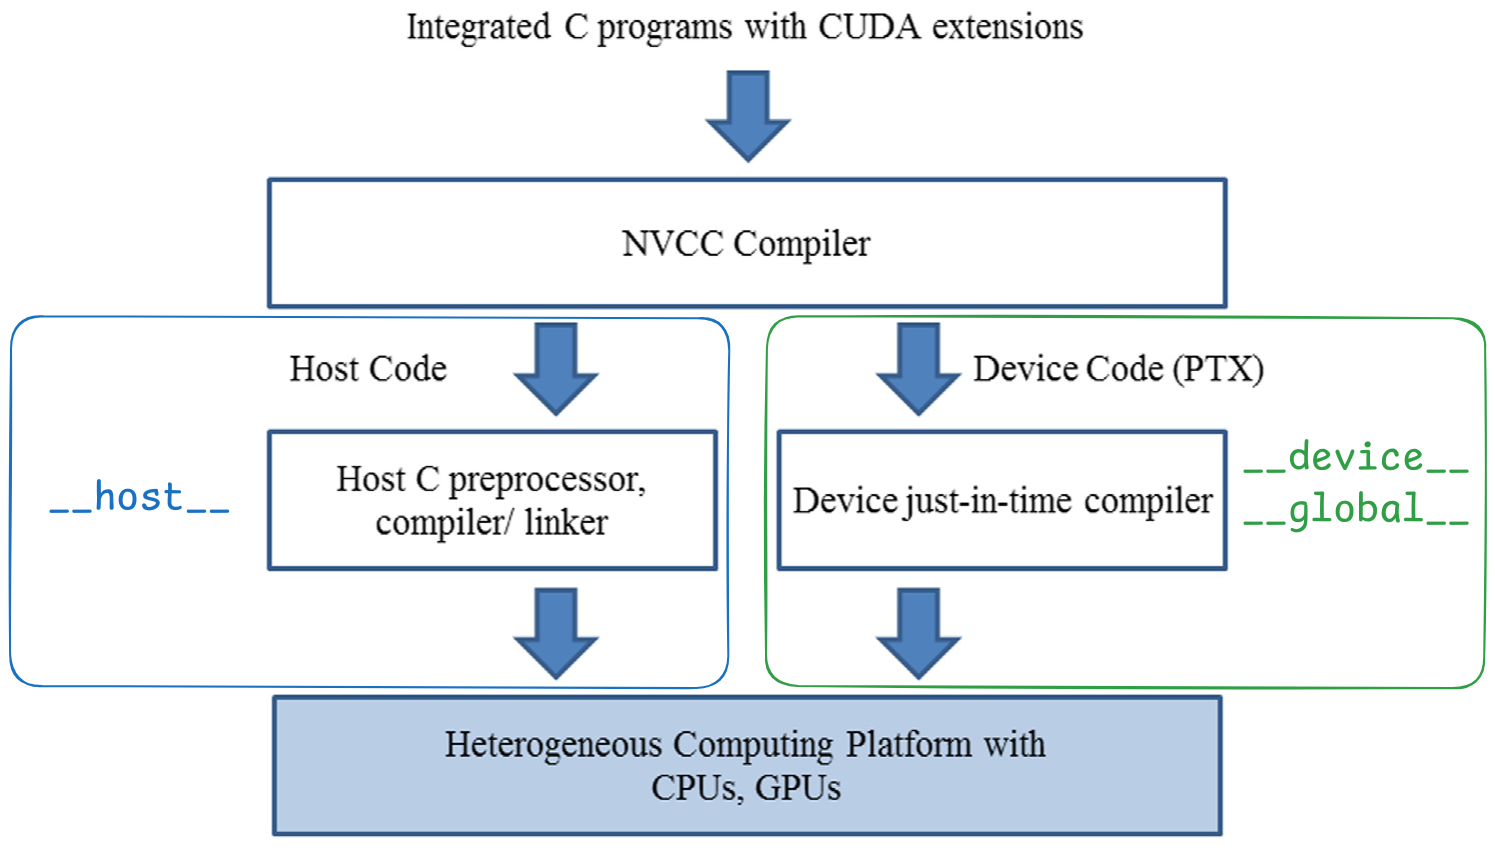
\includegraphics[width=0.7\linewidth]{Images/DP/compilation.png}
\end{center}
\pagebreak